\documentclass[a4paper,english,12pt]{article}
\usepackage{graphicx}
\usepackage[T1]{fontenc}
\usepackage[utf8]{inputenc}
\usepackage{babel}
\usepackage[colorlinks=true]{hyperref}
\usepackage{upgreek} %proper greek letters
\usepackage{fullpage}
\usepackage{lineno}
\usepackage{amsmath} % typesetting math
\usepackage{amssymb}
\usepackage{textcomp}
\usepackage{booktabs} % nice tables
\usepackage[round,sort&compress]{natbib}
\usepackage{pdfpages} %include external pdfs
\usepackage{enumitem} %for noitemsep in lists
\usepackage{csquotes}
\usepackage{subfig}
\renewcommand{\arraystretch}{1.2} % space in tables
\usepackage{authblk}
\usepackage{multirow}
\usepackage{soul}
\usepackage{amssymb}
\usepackage{sidecap}

\newcommand{\mr}[2]{\multirow{#1}{*}{#2}}
\newcommand{\mc}[3]{\multicolumn{#1}{#2}{#3}}

\newcommand{\qq}[1]{\enquote{#1}}

% Comments
\newcommand{\ds}[2][orange]{\textcolor{#1}{#2}}
\newcommand{\bh}[2][red]{\textcolor{#1}{#2}}
\newcommand{\et}[2][blue]{\textcolor{#1}{#2}}

% abbreviations
\newcommand\FOV{\textrm{Res}}
\newcommand\MPS{\textrm{MPS}}
\newcommand\KES{\textrm{KES}}
%\newcommand\du{\textrm{du}}
\newcommand\du{}
\newcommand\DE{\textrm{Eff}}

\begin{document}

\title{Analytical and Monte-Carlo modeling of Multi-Parallel Slit and Knife-Edge Slit Prompt Gamma Cameras}

\author[1,2]{Brent F. B. Huisman}
\author[2]{\'E. Testa}
\author[3]{D. Dauvergne}
\author[1]{J.~M. L\'etang}
\author[1]{D. Sarrut}
\affil[1]{~CREATIS, Universit\'e de Lyon; CNRS UMR5220; INSERM U1206; INSA-Lyon; Universit\'e Lyon 1; Centre L\'eon B\'erard, Lyon, France}
\affil[2]{~Univ. Lyon, Univ. Claude Bernard Lyon 1, CNRS/IN2P3, IP2I Lyon, F-69622, Villeurbanne, France.}
\affil[3]{~ LPSC, Laboratoire de Physique Subatomique et de Cosmologie, CNRS/IN2P3, Université Grenoble-Alpes, Grenoble, France}
\affil[ ]{~E-mail: e.testa@ipnl.in2p3.fr}

\maketitle

\begin{abstract}

\emph{Purpose:}

\emph{Materials and Methods:}

\emph{Results:}

\emph{Conclusion:}

\end{abstract}

\tableofcontents

\newpage

%%%%%%%%%%%%%%%%%%%%%%%%%%%%%%%%%%%%%%%%%%%%%%%%%%%%%%%%%%%%%%%%%%%%%%%%%%%%%%%%
\section{Introduction}

The well-defined range of particles in matter is the main reason they are used in cancer treatment today. Unfortunately we are not able to take full advantage of this property, because of treatment uncertainties, e.g. uncertainties in patient positioning, changes of patient anatomy between treatment fractions and uncertainties in the Hounsfield unit to particle stopping power conversion \citep{Paganetti2012}. Often, medical practice leads to the use of several irradiation fields to ensure robust treatment planning at the expense of larger healthy tissue volume irradiation in respect to ideal treatment with single irradiation field. Moreover margins around the tumor are added, reducing the potential benefits of particle treatment \citep{Knopf2013}. Ion-range verification could permit more precise planning which could take maximum advantage of the steep Bragg peak (BP) fall-off and reduce damage to tissues surrounding the tumor. A promising modality to perform this verification consists in detecting prompt gammas (PGs), a natural byproduct in particle treatments \citep{Krimmer2017a, Parodi2018}. Various modalities are currently under investigation and can be classified in two categories: imaging devices using either mechanical or electronical collimation (respectively collimated \citep{Perali2014, Min2012, Pinto2014a} and Compton cameras \citep{Krimmer2015,Kurosawa2012,Thirolf2016,Polf2015,Llosa2016}) and non-imaging devices such as Prompt Gamma Spectroscopy (PGS) \citep{Hueso-Gonzalez2016}, Prompt Gamma Timing (PGT) \citep{Pausch2016} and Prompt Gamma Peak Integral (PGPI) \citep{Krimmer2017}. Regarding cameras using mechanical collimators, two types of designs have been considered: Multi-Parallel Slit (MPS) and Knife-Edge Slit (KES). The latter has been chosen by the IBA group to be prototyped and has been tested clinically with pencil beam scanning \citep{Xie2017}. Both types of collimators provide part or the whole of the one-dimensional PG profile along the beam direction.

To date, three publications \citep{Smeets2016, Lin2017, Park2017} have attempted to compare these two types of collimators with various geometries. Indeed, although they refer to the same KES design from \citep{Perali2014} some geometrical parameters are slightly different in \citep{Lin2017, Park2017} (i.e. the source-collimator distance and the collimator-detector distance). The same applies for the MPS design: \cite{Smeets2016} uses a modified MPS design from \cite{Pinto2014a}, \cite{Lin2017} used the design from \cite{Gueth2013} and \cite{Park2017} their own specific design. It is worth to note that the authors of the latter publication justified the need for a complementary study by the fact that the MPS geometries used in \cite{Smeets2016, Lin2017} were not \qq{optimized}.
Unfortunately the fact that the optimizations of KES and MPS designs were not performed according the same figures of merit can not ensure a fair comparison of the two designs. Actually from a general point of view the design of any collimated device is a compromise between detection efficiency and spatial resolution. While collimator features have been extensively investigated in the context of nuclear imaging \citep{Gunter2004}, no theoretical considerations have been proposed for the specific 1D collimation systems developed in the context of ion-range verification during hadrontherapy.
Therefore, the first objective of this article is to present an analytical model based on geometrical considerations that allows for a theoretical estimation of the detection efficiency and spatial resolution, for both MPS and KES designs. The intrinsic features of MPS and KES collimators are then derived and the model is validated by means of Monte Carlo (MC) simulations. In light of the predictions of this analytical model, the PG prototypes developed by the CLaRyS collaboration \citep{Pinto2014a, Krimmer2015} and the IBA group \citep{Perali2014} are compared and their performance are assessed in terms of detection efficiency, spatial resolution and fall-off retrieval precision thanks to MC simulations.

%%%%%%%%%%%%%%%%%%%%%%%%%%%%%%%%%%%%%%%%%%%%%%%%%%%%%%%%%%%%%%%%%%%%%%%%%%%%%%%%

\section{Materials and Methods \label{sec:MM}}

\subsection{Analytical model for spatial resolution and detection efficiency}

Camera performance is mainly characterized by a compromise between spatial resolution and detection efficiency. During camera design, modifications of some geometrical parameters, such as collimator-detector distance, collimator pitch or depth, often lead to improvement of one of the criteria and deterioration of the other. We derive an analytical model that predicts camera performance based on the main geometric parameters of collimation. This model can be used to estimate performance according to variation in the geometrical parameters, assuming perfect and full gamma absorption on the absorber entrance surface. Figure~\ref{fig:CamerasParameters} presents the fundamental design of the MPS and KES cameras in tersm of their geometrical parameters, defined in table~\ref{table:CamerasParameters}.

\begin{figure}[htbp]
    \centering
    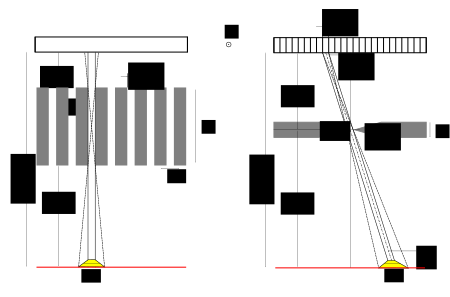
\includegraphics[width=.8\textwidth]{MPS-KES_scheme}
    \caption{Schemes of the Multi-Parallel Slit (MPS) and the Knife-Edge Slit (KES) cameras. The definition of the various parameters is given in Table~\ref{table:CamerasParameters}. The red line corresponds to a linear source perpendicular to the slit camera planes. $\Lambda$ is the the distance between the source point and the detector entrance surface in the KES via the middle of the collimator slit.}
    \label{fig:CamerasParameters}
\end{figure}

\begin{table}[h]
\centering
\begin{tabular}{lllll}
	\midrule
																& MPS               & KES \\
	\midrule
	Source-collimator distance		& $d_1$             & $d_1'$ \\
 	Collimator-detector distance	& $d_2$             & $d_2'$ \\
	Source-detector distance			& $L=d_1+D+d_2$			& $L=d_1'+d_2'$\\
 	Collimator thickness 					& $D$               & $T$ \\
	Camera pitch									& $p$								& $p'$\\
	Knife-edge slit angle					& --								& $\alpha$\\
	%\cline{2-3}
	Slit width										& $s$ 							& $s$ \\ %\multicolumn{2}{c}{s} \\
	Camera height									& $H$ 							& $H$ \\
	\midrule
\end{tabular}
\caption{Geometrical parameters of the MPS and KES cameras. One can also define the fill factor $f$ of the MPS collimator: $f=(p-s)/p$ (ratio between the septa width and the pitch). Note that the source-collimator distance and the collimator-detector distance are not defined exactly in the same way in the two collimator designs.}
\label{table:CamerasParameters}
\end{table}

\subsubsection{Spatial resolution}

From a geometrical point of view, the spatial resolution, denoted $\FOV_{\du}$, is characterized by the \textit{detector unit field of view}. This is the portion of
the source that can be seen through a single camera unit: a single slit for the MPS and a single detector unit for the KES. The probability of a photon emitted at a
given point along a linear source perpendicular to the slit plane to reach
this detector unit can be described as an isosceles trapezoid whose width of the top segment corresponds to the slit width while the width of the base segment is equal to the sum of the slit width and the penumbra. We defined $\FOV_{\du}$
as the FWHM of this trapezoid, see eq~\ref{eq:fov_mps} and \ref{eq:fov_kes}.

\begin{eqnarray}
  \label{eq:fov_mps}
  \FOV_{\du}^{\MPS} & = & s\left(1+ \frac{d_1}{D}\right) = p(1-f) \frac{D+d_1}{D}, \\
  \label{eq:fov_kes}
   \FOV_{\du}^{\KES} & = & s\left(1+ \frac{d_1'}{d_2'}\right) = \frac{sL}{d_2'}.
\end{eqnarray}

If the collimator transparency is neglected, $\FOV_{\du}$ is fully defined by geometrical parameters, in particular the slit width $s$. However, prompt gamma have high penetration capability that can not be neglected in the case of KES where the collimator depth is very small in the region of the knife edge around the slit. Indeed, we define the \textit{Effective Slit Opening} $s_e$ that can be used in the evaluation of the field of view and the efficiency in place of the geometrical slit width. \cite{Metzler2005}
proposed a method to estimate the effective slit width, specifically to calculate
the spatial resolution accurately. The proposed expressions were based on
one-dimensional cuts through the pinhole geometry and can be applied directly to
a knife-edge geometry without modification. Their approach is for a point source
and dependent on the location of the source within the \FOV. For a source in the
center, it simplifies to eq.~\ref{eq:se} with $\mu$ the linear attenuation
length of the collimator material.

\begin{eqnarray}
  s_e & = & s + \frac{\ln2}{\mu\tan\alpha}   \label{eq:se}, \\
   \FOV_{\du}^{\KES} & = & s_e\left(1+ \frac{d_1'}{d_2'}\right) = \frac{s_eL}{d_2'}.
  \label{eq:fov_kes_se}
\end{eqnarray}

Hence, eq.~\ref{eq:fov_mps} and eq.~\ref{eq:fov_kes_se} represent the spatial resolution of the MPS and KES camera systems according to simple geometrical and gamma attenuation parameters (collimator distances, angle and collimator linear attenuation length). The spatial resolution is expressed in millimeters.

\subsubsection{Detection efficiency}

The probability that a gamma reaches a given detector unit is described by the solid angle $\Omega_D$ of the detector unit in respect to the gamma emission point.

For MPS, the solid angle is composed of the azimuthal angle and the polar angle. With small angle approximation, it is described by eq.~\ref{eq:solid_angle_mps}. Note that this is true only when $\Omega_D$ is limited by the slit width, i.e. the absorber size and the distances (e.g. $L$ and $D$) are such that all photons that cross the collimator impinge on absorber material.

For KES, the solid angle under which a point of the source sees a detector unit depends on the location of the point source, $x$, since the distance between source and detector changes significantly over the field of view of the camera. We
consider the solid angle for a point of the source that is within the central
part of the field of view of the crystal at location $x$ on the detector plane
(the origin of the detector plane facing the center of the slit). Under small
angle approximation, the solid angle is given by eq.~\ref{eq:solid_angle_kes}.

\begin{align}
  \Omega_D^{\MPS} & = \frac{H}{L} \frac{s}{D+d_1} \label{eq:solid_angle_mps}, \\
	\Omega_D^{\KES} & = \frac{H L p'}{\Lambda^3(x)} =  \frac{H p'}{L^2 \left( 1+\frac{x^2}{d_2^{'2}} \right)^{3/2}}. \label{eq:solid_angle_kes}
\end{align}
with $\Lambda$ the distance between the source point and the crystal in the KES.


Since we are interested in extended gamma emission source, let us consider now a linear source in front the cameras (red lines in Figure~\ref{fig:CamerasParameters}). In this case, the camera detection efficiency is determined not only by the point source detection efficiency (PSDE) characterized by $\Omega_D$, but also by the fraction of the source seen by the camera (the FOV factor) $f_{\textrm{FOV}} = \frac{\FOV_{\du}}{p}$ where $p$ is the pitch of the camera. It is, in principle, larger than 1 since cameras are usually designed to see all the source without any hidden regions.

Hence, the detection efficiency of a detector unit ($\DE_{\du}$) and therefore the detection efficiency of the whole camera located in front a linear source perpendicular to  the camera plane can be expressed as:
\begin{align}
	\DE_{\du} = \textrm{PSDE} \times f_{\textrm{FOV}},
\end{align}
with $\textrm{PSDE}$ the detection efficiency for a point-like source that sees a detector through the slit, and $f_{\textrm{FOV}} = \frac{\FOV_{\du}}{p}$ the FOV factor. The detection efficiency of MPS and KES are given by equations~\ref{eq:de_mps} and~\ref{eq:de_kes}, respectively.

\begin{eqnarray}
  \label{eq:de_mps}
  \DE_{\du}^{\MPS} & = & \frac{\Omega_D^{\MPS}}{4\pi} \frac{\FOV_{\du}^{\MPS}}{p}, \nonumber\\
                & = & \frac{1}{4\pi} \frac{H}{L} \frac{s}{D+d_1} p(1-f),
                      \frac{D+d_1}{D} \frac{1}{p} ,\nonumber\\
                & = & \frac{Hs(1-f)^2}{4 \pi L D} ;
\end{eqnarray}

\begin{eqnarray}
  \label{eq:de_kes}
	\DE_{\du}^{\KES} & = & \frac{\Omega_D^{\KES}}{4\pi} \frac{\FOV_{\du}^{\KES}}{p'}, \nonumber\\
	& = & \frac{s_e H}{4\pi d_2' L} \frac{1}{\left( 1+\frac{x^2}{d_2^{'2}}\right)^{3/2}}.
\end{eqnarray}

\begin{table}[h]
\centering
\begin{tabular}{lll}
	\midrule
	                            & MPS                              & KES \\
	\midrule
	Effective slit width ($s_e$)& $s$                              & $s + \frac{\ln(2)}{\mu \tan(\alpha)}$ \\
 	Spatial resolution (Res)		& $s \left(1+\frac{d_1}{D}\right)$ & $s_e \left( 1+\frac{d_1'}{d_2'} \right)$ \\
	Detection efficiency (Eff)	& $\frac{H s}{ 4 \pi L D } (1-f) $ & $\frac{H s_e}{ 4 \pi L d_2' } \left( 1 + \frac{x^2}{d_2^{'2}} \right)^{-3/2} $ \\
 	Collimator effective thickness ($T_e$) & $D\times f$           & $T$ \\
	\midrule
\end{tabular}
\caption{MPS and KES detection efficiencies and spatial resolutions from the analytical model. The parameters of the cameras are defined in figure~\ref{fig:CamerasParameters}. $\mu$ is the linear attenuation length of the collimator material.}
\label{table:AMformulas}
\end{table}

In summary, the formulas of detection efficiency and spatial resolution of MPS and KES cameras are gathered in Table~\ref{table:AMformulas}.

Let us define the following conditions that we will refer to as \qq{MPS and KES Similar Conditions} (MKSC):
\begin{itemize}
	\item same distance between the source and the MPS collimator entrance and between the source and the middle of the KES collimator: $d_1=d_1'$ ;
	\item MPS collimator thickness equal to the KES collimator-detector distance: $D=d_2'$ ;
	\item same source-detector distance $L$ (which entails $d_2=0$ with the previous conditions), same height $H$ and same slit width $s$.
\end{itemize}
Let us define the perfect collimator condition (PCC) for which the collimators have infinite absorption capacity. In this condition, $s_e=s$ and the filling factor $f$ of the MPS can be decreased down to zero without degrading the collimation properties.

Combining these two conditions, MKSC and PCC, MPS and KES have strictly the same spatial resolution (Res) and the same detection efficiency (Eff) in the central part of the cameras ($x=0$). The main deviations with the actual MPS and KES performance are the following:
\begin{itemize}
	\item the partial transparency of the collimators leads to:
	\begin{itemize}
		\item an effective slit width of KES larger than the one of the MPS. In the case of the KES prototype of the IBA group using a tungsten alloy collimator (density of 18.5~g/cm$^3$), the term accounting for collimator transparency $\left(\frac{\ln(2)}{\mu \tan(\alpha)}\right)$ is about 5~mm (with $\mu\sim 8\times10^{-1}$~cm$^{-1}$ in the 3-6~MeV range and $\alpha=63$\textdegree) meaning that the effective slit $s_e$ is about twice the actual slit width ($s=6$~mm).
		\item an actual fill factor that cannot be neglected: in the case of the MPS prototype of the CLaRyS collaboration it can be adjusted but a standard value is 0.4, leading to an actual detection efficiency about half the one of the perfect MPS collimator with $f=0$.
	\end{itemize}
	\item the KES design intrinsically leads to a detection efficiency that decreases when the source moves away from the center of the camera while the MPS detection efficiency remains constant over the whole camera field of view.
\end{itemize}

Note that the partial transparency of the collimators leads to an increase of the KES spatial resolution (Res) and a decrease of the MPS detection efficiency (Eff) with similar amplitudes (factor of 2). Since both Res and Eff are proportional to the slit width $s$, one can expect that KES and MPS designs fulfilling MKSC should have very close actual performance if the KES slit width corresponds to the half of the MPS slit width.

For illustration purposes, figure~\ref{fig:AMpredictions} shows the analytical model predictions for the MPS and KES designs compared in \citep{Smeets2016, Lin2017, Park2017}. Parameters have been extracted from the publications (Table~\ref{table:ParametersInLiterature}). We can observe the compromise between detection efficiency and spatial resolution: the designs chosen in these comparisons lead to $\DE_{\du}^{\KES}$ and $\FOV_{\du}^{\KES}$ larger than MPS ones by factors ranging from $\sim3$ to $\sim7$. The detection efficiency obtained by \cite{Park2017} is much larger than the other ones due to camera height ($H$) increase by a factor of 2.

\begin{figure}[!htp]
  \centering
	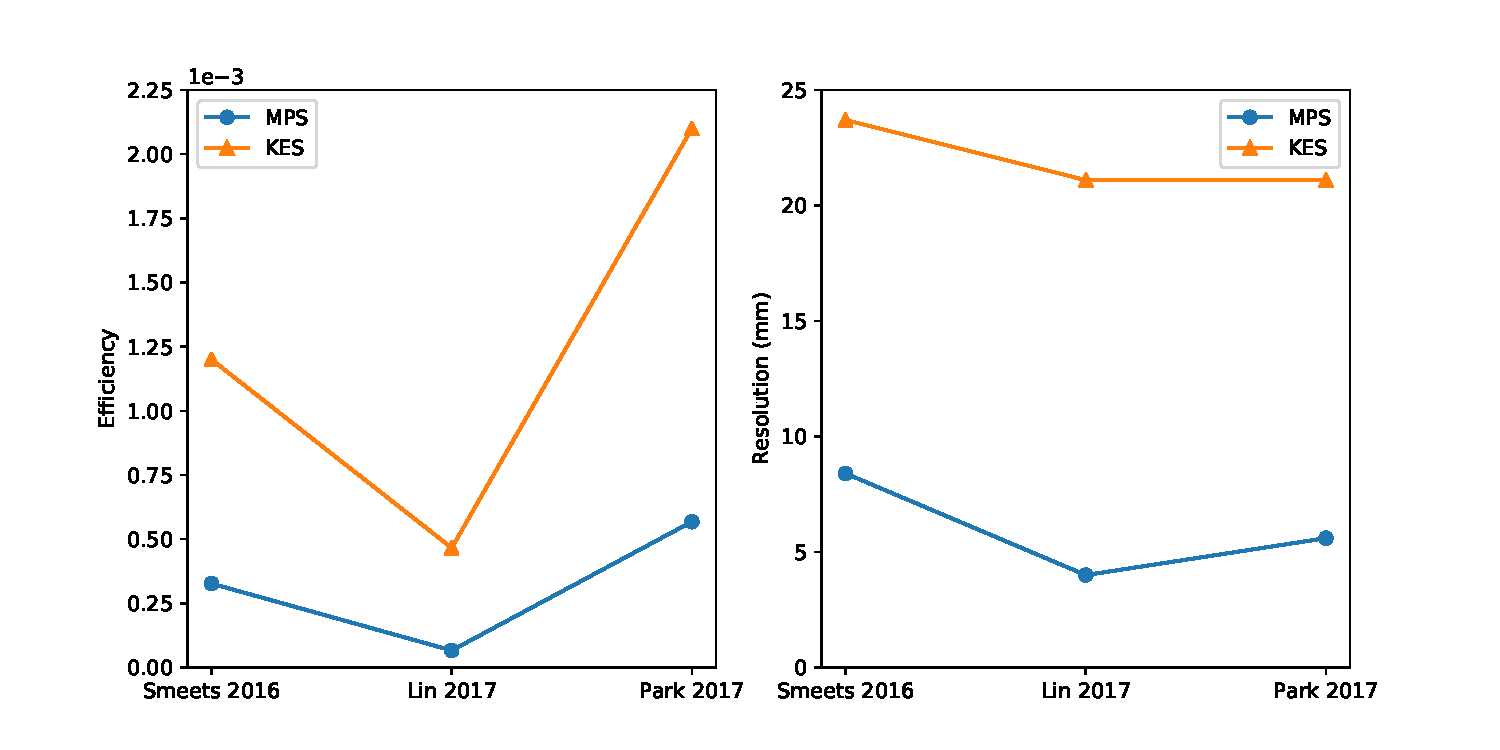
\includegraphics[width=1\linewidth]{./figures/Literature}
  \caption{\label{fig:AMpredictions} Analytical model predictions for the MPS and KES designs compared in \citep{Smeets2016, Lin2017, Park2017}.}
\end{figure}

\begin{table}[h]
\centering
\begin{tabular}{ccccccccccc}
	\hline
	\mc{2}{c}{Parameters}	&& \mc{2}{c}{\citep{Smeets2016}}	&& \mc{2}{c}{\citep{Lin2017}}	&& \mc{2}{c}{\citep{Park2017}} \\
	\cline{1-2}\cline{4-5}\cline{7-8}\cline{10-11}
	MPS	& KES							&&	MPS	& KES	 										&&	MPS	& KES									&&	MPS	& KES					 \\
 	\hline
	$d_1$	& $d_1'$				&& 250	&	220	        						&& 200	& 300					        && 180	& 200	\\
	$d_2$	& $d_2'$				&& 0		&	176	        						&& 200	& 300					        && 0		& 200	\\
	$L$		& $L$						&& 350	&	396	        						&& 600	& 600					        && 280	& 400	\\
	$D$		& $T$						&& 100	&	40	        						&& 200	& 40					        && 100	& 40	\\
	$s$		& $s$						&& 2.4	&	6		        						&& 2		& 6					       		&& 2		& 6	\\
	$H$		& $H$						&& 100	&	100	        						&& 100	& 100				       		&& 200	& 200	\\
	$f$		& 							&& 0.4	&			        						&& 0.5	& 					       		&& 0.5	& 	\\
	\hline
\end{tabular}
\caption{Parameters values of the MPS and KES designs compared in \citep{Smeets2016, Lin2017, Park2017}. All values are in millimeters except $f$ without unit.}
\label{table:ParametersInLiterature}
\end{table}

%%%%%%%%%%%%%%%%%%%%%%%%%%%%%%%%%%%%%%%%%%%%%%%%%%%%%%%%%%%%%%%%%%%%%%%%%%%%%%%%

\subsection{Monte Carlo simulations}
\label{sec:MC}

We compare the analytical model with MC simulations. We estimate, to first order, the intrinsic efficiency of the MPS and KES absorbers with the Beer-Lambert law assuming that a photon is detected as soon as it reaches the detector. At 4~MeV, the MPS absorber of the CLaRyS collaboration and the KES absorber of the IBA group have intrinsic efficiencies of 56\% and 57\% (respectively 3~cm thick BGO scintillators and 3~cm LYSO scintillators).

The objective of MC simulations is twofold: analytical model verification (AMV) and comparing the MPS and KES prototypes. These two studies use slightly different setups that will be detailed in the following subsections.

\subsubsection{Simulation tool}\label{sec:SimTool}

Imaging paradigms such as PG detection are evaluated against experiments, and often also with Monte Carlo (MC) simulations~\citep{Moteabbed2011,Gueth2013,Robert2013,Golnik2014a,Janssen2014}.
For rarely occurring processes such as PG simulation, convergence of MC simulations to within acceptable statistical error can be slow. Therefore, we used in this study the vpgTLE variance reduction method described in \cite{Huisman2016}. vpgTLE is a two-stage process, where firstly a PG yield distribution image is estimated, which in the second stage is used as a PG source. Gate 7.2~\citep{Sarrut2014} with Geant 4.10.02 and the QGSP\_BIC\_HP\_EMY physics list, commonly used for PG studies, are used in this work. Thanks to vpgTLE, simulations for about $10^9$ protons (about $6\times10^8$ photons) took 1-2 hours on a single core of an Intel(R) Core(TM) i7-3740QM.

\subsubsection{Prototypes comparison}\label{sec:camera} % paragraph

The MPS and KES prototypes are illustrated in Figure~\ref{fig:detectors}.

\begin{SCfigure}[][htp]
  \centering
  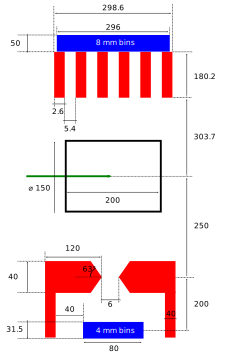
\includegraphics[width=0.5\linewidth]{detectors_cyl2}
	\caption{Schematic presentation of the two PG cameras considered in this study. All distances are in millimeters. The green arrow represents the proton beam. In red the collimation elements and in blue the detection elements. The dimensions were taken from \cite{Pinto2014a} and \cite{Perali2014,Sterpin2015}. Note that the two cameras have an identical height of 200~mm and that here they are not drawn to scale. The magnification factor of the KES prototype is 0.8.}
  \label{fig:detectors}
\end{SCfigure}

\paragraph{The MPS prototype developed by the CLaRyS collaboration.}

This camera intends to measure the whole PG profile to control ion-ranges in the patient with a field of view (FoV) of 300 mm. It consists of a bismuth germanium oxide (BGO) absorber and a tungsten alloy collimator. Each block has a sensitive volume of 3.5$\times$3.8$\times$3 cm$^{3}$ and is streaked in 8$\times$8 pseudo-pixels of 4~mm in edge. In the optimization carried out by \cite{Pinto2014a}, parameters such as collimator pitch, axis-to-collimator and axis-to-detector were varied, and their impacts evaluated in terms of fall-off retrieval precision (FRP) and spatial resolution (sharpness of the fall-off region). Here, configuration 1 of their simulations (with relaxed constraints on spatial resolution) was chosen for its better FRP performance. One can notice that the pitch of the camera (8~mm) corresponds to an integer number of the BGO pseudo-pixel size (4~mm). The event selection from the gamma energy deposition $E$ in the absorber is $E>1$~MeV. Finally this prototype makes use of TOF selection to reduce the neutron background. For the IBA C230 accelerator with a period of 10 ns, \cite{Pinto2014a} chose a window of 4 ns around the PG maximum, based on experimental TOF spectra. Since the neutron background is essentially constant with the IBA C230 time structure \citep{Pinto2014a}, TOF selection should allow for a $\frac{6~\text{ns}}{10~\text{ns}}=60$\% noise reduction for this specific accelerator.

\paragraph{The KES prototype developed by the IBA group}

The purpose of this camera consists of verifying the BP position with a FoV of 100 mm. It consists of two rows of 20 LYSO blocs of 4~mm ($p'$) $\times 100$~mm ($H/2$) $\times30$~mm (thickness) and a tungsten alloy collimator \citep{Perali2014,Sterpin2015}. The standard energy selection for this prototype is $3<E<6$~MeV.

\paragraph{Detector modeling}

The detectors of the two prototypes use different scintillators (absorbers), photodetectors and data acquisition system. In this study, the latter two are not implemented, thus the detector is reduced to its absorber. These are modeled as monoblocks in which the event positions are stored in histograms with bins corresponding to the pitch of the cameras (8~mm for MPS and 4~mm for KES). When a gamma interacts with the absorber, an event is recorded if the integrated energy deposited in the absorber lies in the acceptable energy and TOF windows. Then the energy weighed barycenter of all interactions in the absorber is computed and the event position is assigned to the center of the bin where lies the energy weighed barycenter.

We compared the MPS and KES prototypes with their published properties: $E>1$~MeV and TOF for MPS and $3<E<6$~MeV without TOF for KES. For the sake of completeness and to facilitate the interpretation of the camera performance, several combinations of energy and TOF selections will be studied as well.

\et{To be updated according to Results section}

\subsubsection{Analytical Model Verification (AMV)}

In order to allow for a direct comparison of MC simulations with the analytical model, simulations with perfect collimators (PCC) and detectors will be performed. This camera version we refer to as \qq{perfect camera}, while the unchanged version will be referred to as \qq{physical camera}. Table~\ref{tab:CameraParameters} gives an overview of the cameras main parameters used for AMV and prototypes comparison.

\begin{table}[h]
\centering
\begin{tabular}{|l|l|l|l|}
	\hline
	\mc{2}{|c|}{}												& Prototypes comparison (PC)			& 	Analytical model verif. (AMV)\\
	\hline
	\mr{2}{Absorber}							& MPS & BGO 														& \mr{2}{Perfect} 							\\
	\cline{2-3}
																& KES & LYSO 														& 																\\
	\hline
		\multicolumn{2}{|l|}{Collimator} 	& Tungsten alloy 									& Perfect							\\
	\hline
	Energy 												& MPS &		>1 MeV												& \mr{2}{>1 MeV}									\\
	\cline{2-3}
	selection											& KES & 3--6 MeV 												& 																\\
	\hline
	TOF 													& MPS &		TOF														& \mr{2}{no TOF}									\\
	\cline{2-3}
	selection											& KES & no TOF 													& 																\\
	\hline
	\mc{2}{|c|}{BKGD modeling} 					& Exp. data based modeling  			& No modeling  \\
	\hline
	\multicolumn{2}{|l|}{Target} 				& Cylindrical PMMA phantom    		& No 															 \\
	\hline
	\multicolumn{2}{|l|}{Beam} 					& \mc{2}{c|}{160 MeV proton}   \\
	\hline
	\multicolumn{2}{|l|}{Number of particles} 				& $10^7$, $10^8$, $10^9$    		& $10^9$ 															 \\
	\hline
\end{tabular}
\caption{Summary of the cameras main parameters used for AMV and PC. The configuration of the column \qq{Prototypes comparison} corresponds to the reference one with standard energy and TOF selections. In the case of AMV, the gamma source corresponds to the PGs emitted during the PMMA phantom irradiation with 160 MeV proton beam (first stage of the simulation tool, see section~\ref{sec:SimTool}). However the target has been removed in the second stage of the simulation tool (PG detection) to avoid any attenuation and allow for a direct comparison of the detection efficiency with the AM predictions.}
\label{tab:CameraParameters}
\end{table}

\subsubsection{Background modeling}\label{sec:BKGD}

\paragraph{Prototypes comparison}

Background (BKGD) estimation in PG simulation is a difficult and still an unsolved issue \citep{Huisman2016,Sterpin2015,Pinto2014a,Perali2014}. Simulations would ideally include beam nozzle and whole room modeling, but these are habitually omitted. TOF selection techniques can improve the signal-to-noise ratio (SNR) \citep{Testa2008,Roellinghoff2014a}, but then it depends on the proper simulation of the beam accelerator time structure. As noted in \cite{Huisman2016}, no validation for background in PG simulations has been performed at this time. In this study, we considered the IBA C230 accelerator time structure in which the neutron background is essentially constant. The estimates of background counts in the detector were taken from \cite{Pinto2014a,Perali2014} and are given in Table~\ref{tab:BKGD}.

\begin{table}[h]
\centering
\begin{tabular}{lcc}
	\toprule
		& MPS			& KES \\
	\midrule
	Bin width (mm) (pitch)	& 8				& 4 \\
	BKGD counts per bin			& 250			& 500 \\
	BKGD level per mm				& $\sim30$& $\sim120$ \\
	\bottomrule
\end{tabular}
\caption{Background (BKGD) counts for $10^9$ incident protons estimated from Figure~9 of \cite{Pinto2014a} for MPS and from Figure~11 of \cite{Perali2014} for KES. The energy and TOF selections are given in Table~\ref{tab:CameraParameters} (column \qq{Prototype comparison}).}
\label{tab:BKGD}
\end{table}

% For reference for above table:
% \item MPS: \cite{Pinto2014a} $1 \cdot 10^{3} \pm 1 \cdot 10^{2}$ per $4\cdot10^9$ primary protons per 8 mm bin (Figure~9)
% \item[] Converted to per primary proton: $2.5 \cdot 10^{-7} \pm 0.25 \cdot 10^{-7}$
% \item KES: \cite{Perali2014} $5 \cdot 10^{-7} \pm 0.5 \cdot 10^{-7}$ per primary proton per 4 mm bin (Figure~11)

Per unit of bin length, the background yield of the MPS with TOF is therefore 4 times as low as the background seen with the KES (without TOF). For the KES camera the background with TOF can be obtained by multiplying the background with the same $\frac{4 ns}{10 ns} = 0.4$ fraction as with the MPS.

\paragraph{Analytical Model Verification}

For the AMV, the background will be left out, as only gamma detection is modeled.

\subsubsection{Beam and target}

\paragraph{Prototypes comparison}

We use the test-case presented in \cite{Perali2014} because the KES detector properties, such as the background, were published for that scenario, again in order to remove any doubt that a difference in camera performance could be due to a difference in implementation or setup. A 160 MeV mono-energetic proton beam is shot into a cylindrical PMMA phantom (length 30 cm, radius 15 cm). Employing the batch method we performed 50 simulations for each experiment.

\paragraph{Analytical Model Verification}

In the case of AMV, the same source is used (first stage of the simulation tool, see section~\ref{sec:SimTool}). However the target has been removed in the second stage of the simulation tool (PG detection) to avoid any attenuation and allow for a direct comparison of the detection efficiency with the AM predictions.

%%%%%%%%%%%%%%%%%%%%%%%%%%%%%%%%%%%%%%%%%%%%%%%%%%%%%%%%%%%%%%%%%%%%%%%%%%%%%%%%
\subsection{Figures of merit}\label{figmerit}

\subsubsection{Analytical Model Verification}

The comparison of the analytical model with Monte Carlo simulations will be performed on the two features predicted by the model: the detection efficiency and the spatial resolution. These quantities can be derived from the Monte Carlo results as follows:

\begin{itemize}
	\item The detection efficiency is computed as the ratio of the mean number of detected gammas over the number of emitted gammas for camera units seeing the PG profile.
	\item The spatial resolution is derived from the fall-off width (\textbf{FOW}) of the simulated PG profiles. We define this width as the FWHM of the peak resulting from the computation of the PG profile first derivative.
\end{itemize}
\subsubsection{Prototypes Comparison}

In addition to the figures of merit mentioned for AMV, the fall-off retrieval precision (\textbf{FRP}) will be determined for its clinical relevance. The FRP is the standard deviation of the fall-off position (\textbf{FOP}) distribution, which is obtained by way of the batch method. Each of these can then be examined as function of the energy and TOF selections. A comprehensive description of our procedures for retrieving the FOP, FOW and FRP is provided in appendix~\ref{sec:fopproc}.

%%%%%%%%%%%%%%%%%%%%%%%%%%%%%%%%%%%%%%%%%%%%%%%%%%%%%%%%%%%%%%%%%%%%%%%%%%%%%%%%
\section{Results}

\subsection{Analytical Model Verification}

Figure~\ref{fig:PGprofileFairComp} shows PG profiles obtained with MPS and KES with perfect detector, the same energy E>1~MeV and no TOF selection.

\begin{figure}[!htp]
  \centering
  \subfloat[MPS]{\label{SmeetsComparison}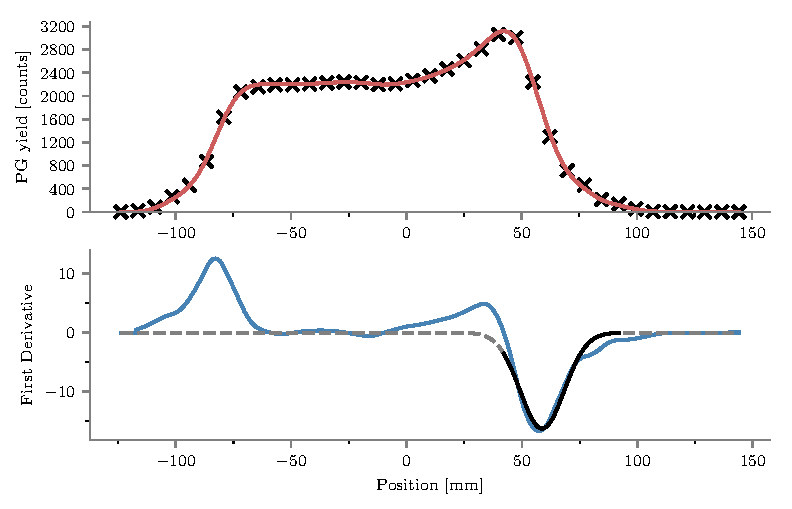
\includegraphics[width=.45\textwidth]{amv_mps_fow}}\quad
  \subfloat[KES]{\label{LinComparison}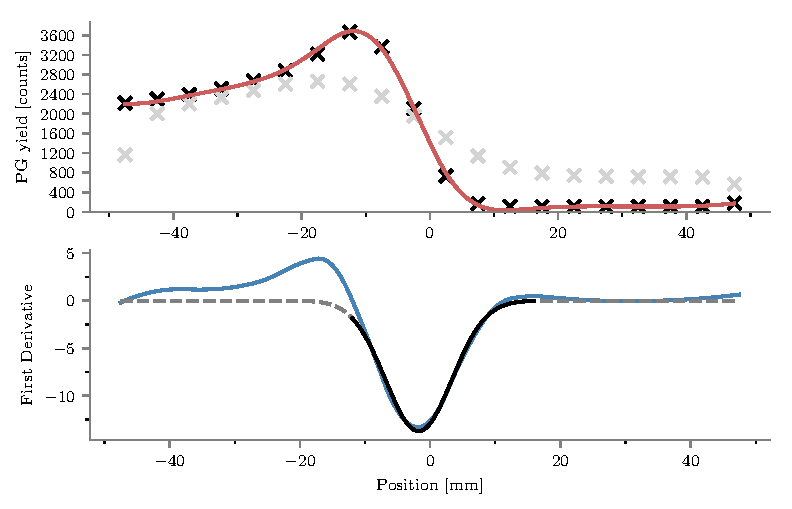
\includegraphics[width=.45\textwidth]{amv_kes_fow}}
  \caption{\label{fig:PGprofileFairComp} PG profiles obtained with MPS and KES prototypes with perfect collimator and detector, the same energy (E>1 MeV) and no TOF selection (analytical model verification). The first row shows the datapoints in black crosses with the curvefit in red. The points in light gray are the data from the physical detector for otherwise the identical simulation. On the bottom row the first derivative of the red fit is shown, with the dashed line the Gaussian fit over the fall-off region (solid). The spatial resolution of the cameras is defined as the FWHM of this Gaussian fit.}
\end{figure}

\begin{table}[h]
\centering
\begin{tabular}{lllllllll}
	\midrule
	\multicolumn{2}{c}{}				& \multicolumn{3}{c}{MPS}																	&& \multicolumn{3}{c}{KES}										\\
	\cline{3-5}\cline{7-9}
	\multicolumn{2}{c}{}				& AM 										& MC 									& RD	 			&& AM 										& MC & RD							\\
	\midrule
	Res	& Perfect camera				& 14.5 								& 15.3  	 			& 5.2 \%	&& 13.5 								& 18.3 				& 26 \%  \\
	(mm)	& Phys. camera					& 					& 17.3  	 					&						&& 23.7									& 28.0 									& 15 \% \\

	\midrule
	Eff    & Perfect camera			&  $6.66 \cdot 10^{-4}$ & $6.48\cdot10^{-4}$	&	3 \%					&& $1.06 \cdot 10^{-3}$  & $1.65\cdot10^{-3}$			& 36 \%\\
	       & Phys. camera				&  $3.76 \cdot 10^{-4}$	& $4.60\cdot10^{-4}$	&	18 \%					&& $6.03 \cdot 10^{-4}$	& $1.28\cdot10^{-3}$	& 52 \%\\
 	\midrule
	FRP    & Perfect camera			&  & 0.13 	&  &&  & 6.7 	\bh{?}		& \\
	(mm)       & Phys. camera				&  & 0.30 	&  && 	& 0.28 	& \\
 	\midrule
\end{tabular}
%FRP = fopsigma
%Res = fow
%Eff = detcount/prod
\caption{MPS and KES detection efficiencies (\qq{Eff}) and spatial resolution (\qq{Res}) from analytical models and MC. The predictions of the analytical model (AM column) are derived from the equations of table~\ref{table:AMformulas}, at the center of the camera in the case of KES ($x=0$). MC data have been obtained with energy selection E>1~MeV. As mentioned in section~\ref{sec:MM}, the gamma source corresponds the PG distribution generated during the PMMA phantom irradiation with 160 MeV proton beam (first stage of the simulation tool). Then the target has been removed in the second stage of the simulation tool (PG detection) to avoid any attenuation and allow for a direct comparison of the detection efficiency with the AM predictions. RD: relative deviation between AM and MC.}
\label{tab:AMV}
\end{table}

Table~\ref{tab:AMV} compares the detection efficiency and the spatial resolution obtained from the analytical model and Monte Carlo simulations.

Main results:
\begin{itemize}
	\item Very good agreement between AM and MC (perfect cameras) except the discrepancy on the MPS resolution. Good agreement on the KES spatial resolution with physical camera.
	\item The discrepancy on the physical camera efficiency is due to the transparency of the collimators that is not taken into account in the AM.
\end{itemize}

\paragraph{Spatial Resolution} The results for the spatial resolution

\paragraph{Efficiency}

\paragraph{Fall-off Retrieval position} The MC-obtained fall-off retrieval position is also given in table~\ref{tab:AMV}. The model does not predict FRP, but results are given to see the effect of switching from a perfect camera model to the physical one. The closeness of the results implies that for the MPS in particular the opacity of the collimator and quality of PG detection in the detector don't have much room for improvement.

% \begin{figure}[htp]
%   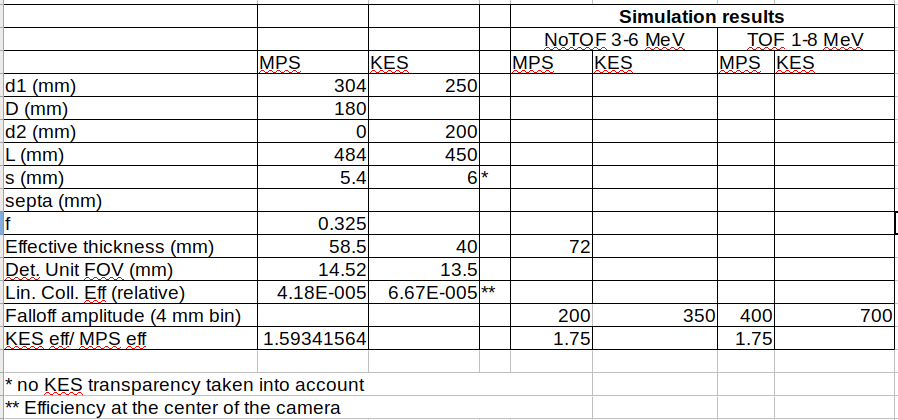
\includegraphics[width=\textwidth]{FairComparison}
%   \caption{\label{CameraperformanceFairComp} MPS and KES comparisons with the same absorber, energy and TOF selection. The first columns of the table correspond to the geometrical calculations. \textcolor{red}{It is interesting to show the results for the two energy selections but it would be nice to have only one TOF selection (no TOF).}}
% \end{figure}

\subsection{Prototype Comparison}

Performance under clinical conditions is the primary purpose of these PG cameras, and therefore we include the results of the clinical case study. As described in table~\ref{tab:CameraParameters}, we took settings and corresponding background estimates for the camera's published settings to simulate each camera as-is during measurements of the same PMMA phantom.

\subsubsection{PG profiles}

Figure~\ref{fig:PGprofileProtoComp} shows the PG profiles with $10^9$ protons, averaged over 50 runs. The averaging removes statistical fluctuations so that the base structure of the profiles can be best studied. The MPS camera is large enough to capture both the fall-off and fall-in positions, so the camera was displaced slightly (5~cm in the distal direction) in order for the full profile to show up. The expected fall-off is at $+50$~mm and 0~mm for the MPS and KES respectively.

\begin{figure}[!htp]
  \centering
  \subfloat[MPS]{\label{SmeetsComparison}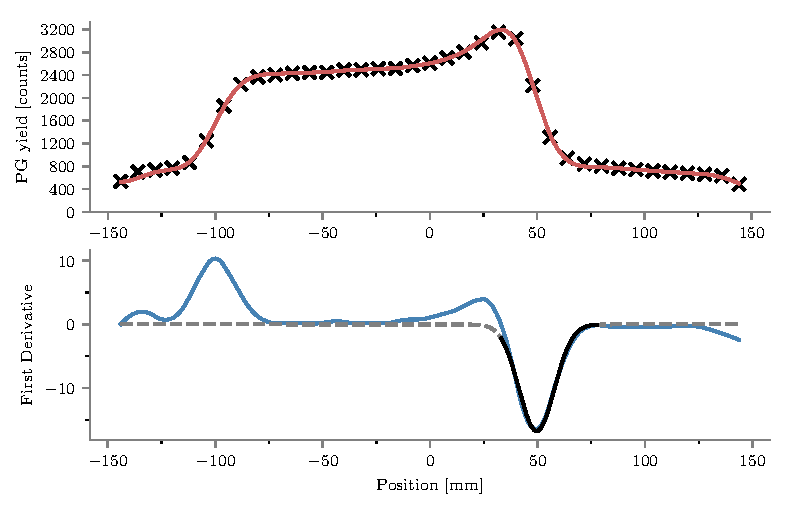
\includegraphics[width=.45\textwidth]{pc_mps_fow}}\quad
  \subfloat[KES]{\label{LinComparison}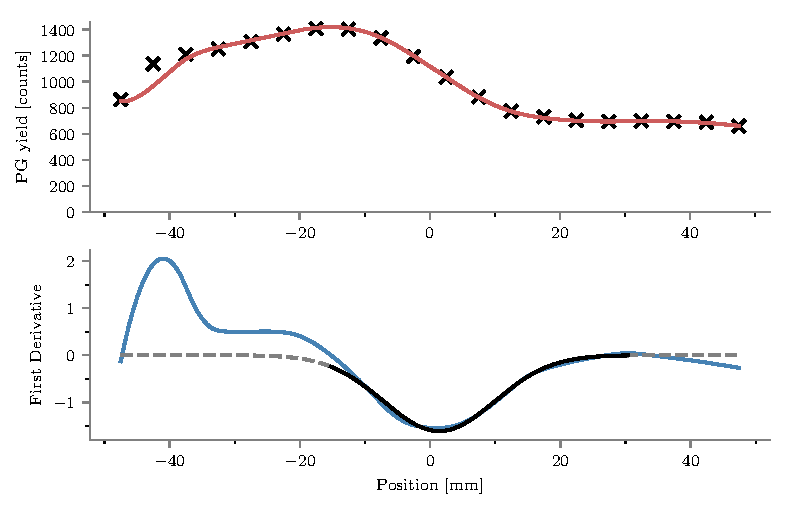
\includegraphics[width=.45\textwidth]{pc_kes_fow}}
  \caption{\label{fig:PGprofileProtoComp}MPS and KES prototypes comparisons. MPS BGO absorber with 1-8 MeV energy selection and TOF selection. KES: LYSO absorber with 3-6 MeV and no TOF selection. On the top row the reconstructed profiles, averaged over 50 simulation each with $10^9$ protons. On the bottom row in blue the first derivative of the profile, with in black the Gaussian fit in the fall-off region, with which the fall-off position and width will estimated. Note that the horizontal scales are different and correspond to each camera's field of view.}
\end{figure}

We can see that, as expected, the MPS has higher PG counts, because of the wider energy selection (the PG production spectrum shows most production at lower energies). We see qualitatively the fall-off positions are at the expected coordinate, and that the BP is more pronounced in the MPS. At the tail end we see the backgrounds converge on roughly the same level.

\et{We expect different \qq{tail levels}:
	\begin{itemize}
		\item Tail level (Figure~\ref{fig:PGprofileProtoComp}) = Tail level without background (Figure~\ref{fig:PGprofileFairComp}) (tail due to collimator partial transparency -- light gray points)+ background level (section~\ref{sec:BKGD}). Table~\ref{tab:Tails} shows the expected tails with and without background: the MPS expected tail with background (650) is in accordance with the PG profile tail in Figure~\ref{fig:PGprofileProtoComp}. However it seems that the background has not been taken into account in the KES PG profile (tail level of $\sim800$ close to the tail without background of Figure~\ref{fig:PGprofileFairComp}).
		\begin{table}[h]
		\centering
		\begin{tabular}{lll}
			\midrule
										& MPS			& KES \\
			\midrule
			Tail wo BKGD (Figure~\ref{fig:PGprofileProtoComp})	& 400			& 800\\
			BKGD level (section~\ref{sec:BKGD}) 	& 250			& 500\\
			\midrule
			Expected tail with BKGD& 650			& 1300\\
			\midrule
			\qq{Observed} Tail in Figure Figure~\ref{fig:PGprofileProtoComp} & $\sim650$			& $\sim800$\\
			\bottomrule
		\end{tabular}
		\caption{\et{Expected background counts (in the tail region) for $10^9$ incident protons. Table to be removed from the paper.}}
		\label{tab:Tails}
		\end{table}
		\item Note that the cameras have different bin sizes (8 mm for MPS and 4 mm for KES). We need to divide the MPS counts by 2 to compare the tail levels.
	\end{itemize}
}


Table~\ref{tab:ProtoPerformance} summarizes the spatial resolution and efficiency results. Even though the MPS had a more pronounced fall-off, we can see the spatial resolutions are roughly equivalent. \bh{Some comment on efficiency?}


\begin{table}[h]
\centering
\begin{tabular}{llllll}
	\midrule
			& MPS					& KES \\
	\midrule
 	Res		& 19.4 mm				& 20.1 mm\\
	Eff  	& $1.04\cdot10^{-3}$	& $5.58\cdot10^{-4}$\\
 	\midrule
\end{tabular}
\caption{Detection efficiencies and spatial resolution of MPS and KES prototypes. Energy and TOF selection: E>1~MeV and TOF for MPS -- 3-6~MeV and no TOF for KES.}
\label{tab:ProtoPerformance}
\end{table}

\subsubsection{FRP}

Figure~\ref{fig:PCFRPComp} shows the falloff retrieval precision (FRP) (standard deviation of the falloff position distributions) for the 2 prototypes as a function of the number of incident protons ($10^7$, $10^8$, $10^9$). As expected, more primaries translate to a better FRP. Both cameras achieve submillimetric accuracy at $10^9$ primaries, and millimetric precision with $10^8$ primaries. With fewer than $10^8$ primaries, the cameras, KES in particular, are outside the limits of interest of shift detection.

\begin{figure}[!htp]
  \centering
  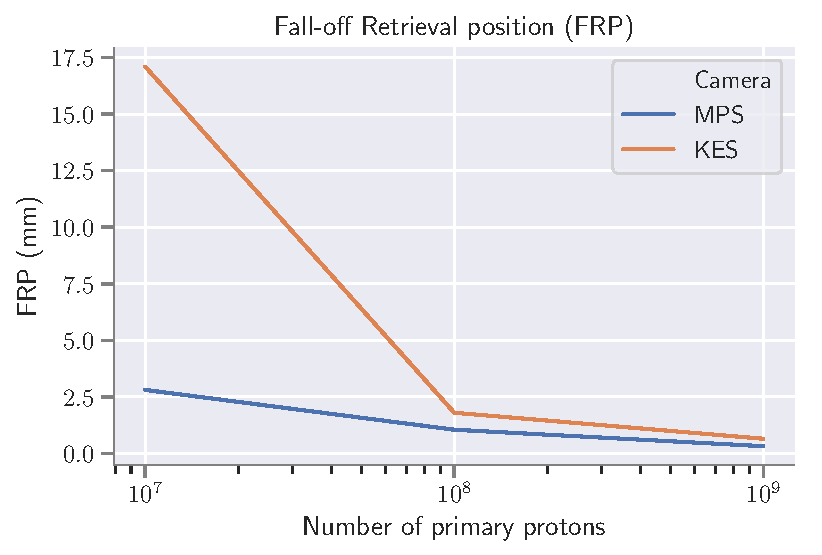
\includegraphics[width=.8\textwidth]{pc_frp_plot}
	\caption{\label{fig:PCFRPComp}Fall-off retrieval precision of the prototypes as a function of the number of incident protons. \et{Remove the title of the figure (which is btw incorrect: FRP= precision and not position).}}
\end{figure}

\et{Figure~\ref{fig:PCFRPComp} does not present all the data of Table 6. Brent, could you try to plot all the data with the following notations?}
	\begin{itemize}
		\item KES (orange), MPS (blue)
		\item Add the points with full symbols (TOF) and open symbols (no TOF)
		\item E>1 MeV (full line) and E>3 MeV (dashed line)
	\end{itemize}
	\et{I think that this set of FRP is important to discuss the performance of the MPS and KES prototypes as a function of energy and TOF selections.}

\begin{table}[h]
\centering
\begin{tabular}{llllllllll}
	\midrule
	Primaries & Time selection 					& TOF &     &     &     & none&     &     &     \\
	          & Energy selection 				& 1   &     & 3   &     & 1   &     & 3   &     \\
	          & Camera 							& MPS & KES & MPS & KES & MPS & KES & MPS & KES \\
	\midrule
 	$10^9$    & AMV perfect det.        & 0.90 & 0.10 & NTNE\\
% 	$10^9$    & AMV perfect det.        & ? & 0.44 & 0.49 & 0.52 & 0.42 & 0.40 & 0.45 & 0.55 \\
% 	$10^8$    & LYSO and no bg        & ? & 1.22 & 1.70 & 1.74 & 1.24 & 1.29 & 1.63 & 1.48 \\
% 	$10^7$    & LYSO and no bg        & ? & 4.03 & 5.88 & 5.65 & 3.76 & 4.89 & 5.65 & 10.76 \\
	\midrule
 	$10^9$    & detectors as proposed     & \textbf{0.32} & 0.56 & 0.36 & 0.57 & 0.31 & 0.60 & 0.46 & \textbf{0.65} \\
 	$10^8$    & detectors as proposed     & \textbf{1.05} & 1.69 & 1.30 & 1.96 & 1.04 & 1.93 & 1.34 & \textbf{1.80} \\
 	$10^7$    & detectors as proposed     & \textbf{2.81} & 7.96 & 3.65 & 12.9 & 2.96 & 14.8 & 19.3 & \textbf{17.1} \\
	\midrule
\end{tabular}
\caption{\bh{THIS TABLE IS TO BE REMOVED. REPLACED WITH FRP PLOT.}Fall-off retrieval precision (defined as the standard deviation of the FOP over the number of times the simulation is ran. In bold, the cuts and TOF selections as proposed.}
\label{FRPCOMP}
\end{table}

%%%%%%%%%%%%%%%%%%%%%%%%%%%%%%%%%%%%%%%%%%%%%%%%%%%%%%%%%%%%%%%%%%%%%%%%%%%%%%%%
\section{Discussion}

Mention the limitations of the KES: detection efficiency not constant over the FOV + limited FOV

\et{I (Etienne) plan to write this section once the Results section is completed.}


\subsection{Clinical implications}

It is often stated PG cameras will be able to be used to track deviations at the spot-level. The cameras in this study required $10^8$ primaries for an acceptable FRP. It is helpful to put this in clinical perspective, so we plot the structure of two treatment plans in figures \ref{fig:planmid} and \ref{fig:planhigh}. These treatment plans were produced and used for two clinical cases, the former considered of medium complexity, which is to say a fairly typical plan, and the second of high complexity. It stands to reason that from a clinical point of view, treatment monitoring becomes more interesting as the complexity of the plan increases, because plans become more complex in more difficult or sensitive cases, where a correct planned and delivered dose are desirable.

\begin{figure}[htp]
  \centering
  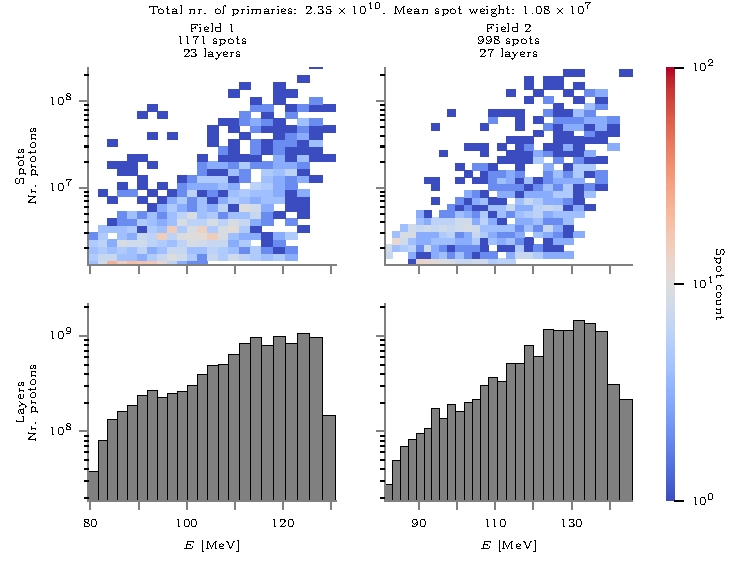
\includegraphics[width=0.8\linewidth]{MENINGIOMA_F1nonorm-plot}
  \caption{Treatment plan for a Meningioma case, which is considered a plan-type of medium complexity. On top: the spots are binned as function of energy and spot weight (number of protons), with high spot counts in red (hot spots) and low spot counts in blue (cool spots).}
  \label{fig:planmid}
\end{figure}

\begin{figure}[htp]
  \centering
  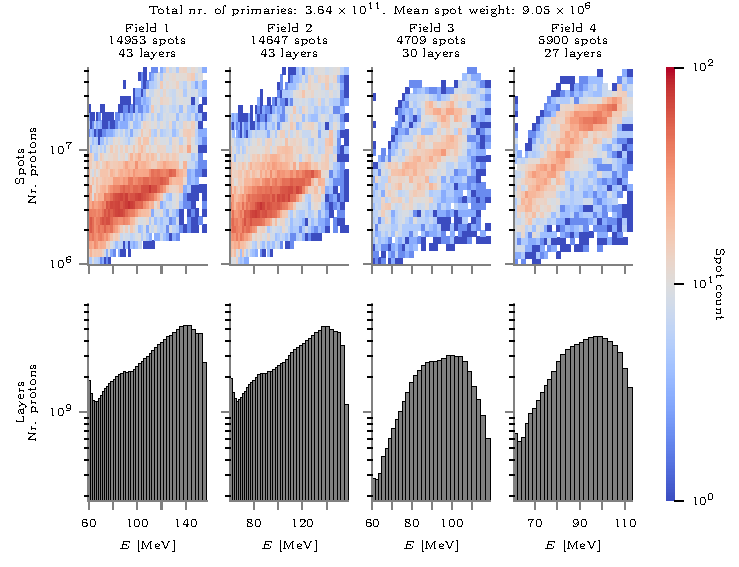
\includegraphics[width=0.8\linewidth]{CSI_F1nonorm-plot}
  \caption{Treatment plan for a large and complex pediatric brain and spine case. The left two fields are for the brain, the right two for the spine. The color scale chosen the same as in figure \ref{fig:planmid}.}
  \label{fig:planhigh}
\end{figure}

From figures \ref{fig:planmid} and \ref{fig:planhigh} we can observe that spot-level monitoring is unlikely with the camera prototypes included in this study. In the complex case not a single spot has a prescription of $10^8$ protons or more. Fortunately, nearly all energy layers exceed $10^8$ primaries, so monitoring at the layer-level poses no issues for these cameras. Nevertheless, we hope the theoretical framework developed and validated in this paper will help move PG camera designs towards the realm where spot-level monitoring would become feasible.

%%%%%%%%%%%%%%%%%%%%%%%%%%%%%%%%%%%%%%%%%%%%%%%%%%%%%%%%%%%%%%%%%%%%%%%%%%%%%%%%
\section{Conclusion}

We have presented and validated an analytical model that relates the collimator dimensions of Prompt Gamma cameras to a predicted spatial resolution and detection efficiency. Two collimator designs are modelled: multi-parallel slit and knife edge. The validation consisted of Monte Carlo simulations of two current Prompt Gamma camera prototypes, one of which has been employed in clinical setting. We also show the performance of these two prototypes in their proposed configuration with a mono-energetic spot in a PMMA phantom with background modelling. The prototypes reach millimetric precision with $10^8$ primaries or more. The fall-off retrieval position performance is put into clinical context.

%%%%%%%%%%%%%%%%%%%%%%%%%%%%%%%%%%%%%%%%%%%%%%%%%%%%%%%%%%%%%%%%%%%%%%%%%%%%%%%%
\section{Acknowledgments}

This work was partly supported by SIRIC LYric Grant INCa-DGOS-4664, LABEX PRIMES (ANR-11-LABX-0063 / ANR-11-IDEX-0007) and Fondation ARC. The authors would like to thank Marie-Claude Biston, Thomas Baudier and Gloria Vilches-Freixas for their help finding the CT images and making the treatment plan. We also thank Erik Almhagen and Uppsala University Hospital, Sweden for the treatment plan data presented in this paper.

%%%%%%%%%%%%%%%%%%%%%%%%%%%%%%%%%%%%%%%%%%%%%%%%%%%%%%%%%%%%%%%%%%%%%%%%%%%%%%%%
\newpage

\appendix
% \begin{appendices}
%
%%%%%%%%%%%%%%%%%%%%%%%%%%%%%%%%%%%%%%%%%%%%%%%%%%%%%%%%%%%%%%%%%%%%%%%%%%%%%%%%

\section{Fall-off position and width estimation procedure}\label{sec:fopproc}

\subsection{Fall-off position estimation procedure}

From a clinical perspective, the range estimate could be more interesting than FOP, because it can distinguish simple offset errors from patient morphological change. While the MPS camera was conceived for whole range PG profile detection, the KES camera FoV was chosen for BP region PG detection only. To make the comparison fair, only the FOP could be considered. Multiple approaches to extracting a FOP from the line profile have been proposed \citep{Smeets2012,Gueth2013,Roellinghoff2014a,Janssen2014,Sterpin2015}. In preparatory work, a number of the proposed procedures were investigated. Significant sensitivity to free parameters on the final FOP estimates were seen. In summary, the FOP estimate depends greatly on the procedure, and often on having yields uncommon on the spot-level in clinical TPs, and also on an absence of unavoidable inhomogeneities.

Therefore the fitting method was not chosen as a topic for study in this paper. Instead, a simple method that works on most the data available to the authors was used: first a smoothed and interpolated spline function is fitted against the detected PG data points, after which a baseline and (distal) peak position are determined. The intersection of the spline with the half-height of the peak above the baseline is then taken as the FOP.


\begin{enumerate}[noitemsep]
\item The measured PG profile is smoothed and interpolated with a smoothing spline function:

\begin{equation}
\sum_{i=1}^n (y_i - \hat f(x_i))^2 + \lambda \int_{x_1}^{x_n} \hat f''(x)^2 \,dx
\end{equation}

where $y_i$ is the measured PG profile and $x_i$ the associated x-coordinates, $\hat f(x_i)$ the estimate smoothed spline function and $\lambda$ a smoothing parameter that determines the penalty for deviating from measurement in exchange for smoothness (second order derivatives are close to zero on smooth functions). $\lambda = 0$ produces a perfect spline fit to the data, while $\lambda \gg 1$ produces a horizontal line. We found that $\lambda = 2$ provided an acceptable trade-off between overfitting to noise and removing too many features, which tends to happen for low statistic measurements.
\item The obtained function is plotted for 1024 $x_j$, an number that provided a sufficiently high resolution. Any $f(x_j) < 0$ are set to $0$.
\item The global maximum is found.
\item The baseline is set equal to the lowest 25\% of bins.
\item From the distal end backwards, the first maximum is taken as the distal most peak position, if it is above the threshold of 30\% of the difference between baseline and global maximum. If no such point is found, the global maximum is taken as the distal most maximum.
\item The fall-off amplitude (FOA) is set to the difference between the distal maximum and baseline: $FOA = max-baseline$. The FOP is obtained by traversing the smoothed profile from the distal end towards the peak until $y_j > \frac{1}{2}FOA$.
\end{enumerate}

The results of this procedure are illustrated in figure~\ref{fig:our-fit}. Every PG profile was estimated 50 times, and so we obtained 50 estimates for the FOP. It is assumed that the FOPs follow a Gaussian distribution, so the mean of the 50 realizations gives the best FOP estimate and the sigma gives the precision of the ability to estimate the best FOP. Comparing the 50 FOP estimates obtained from the CT with the 50 estimates obtained from the RPCT simulations, gives 2500 possible shift estimates. Again, the distribution of shifts should be centered at the true shift, while the sigma indicates how likely it is that this true shift is detected under the current conditions.

\begin{figure}[htp]
  \centering
  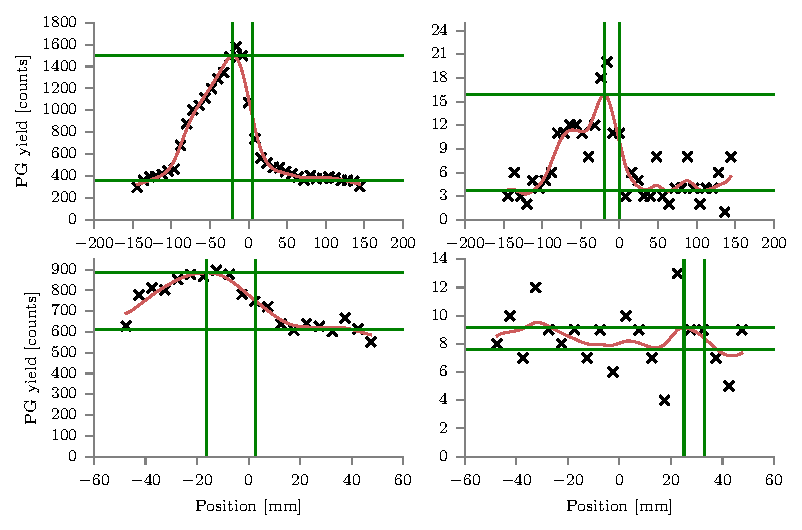
\includegraphics[width=0.9\linewidth]{fopproc}
  \caption{The top row demonstrates the fall-off determination procedure on the multi-parallel camera data; on the bottom row on knife-edge slit camera data. The left column is produced with a PG signal due to $10^9$ primaries, while the right column was produced with $10^7$ primary protons. In black crosses the measured PG counts are plotted. The smoothed data is shown in red. The green horizontal lines are drawn at the obtained distal maxima and baselines, while the vertical green lines shown the position of the distal maximum and the position of the fall-off. For the bottom-right plot, a history is visible where the procedure fails: the background induces an erroneous peak detection.}
  \label{fig:our-fit}
\end{figure}

\subsection{Fall-off width estimation procedure}

\begin{figure}[htp]
  \centering
  \subfloat[KES]{\label{FOWKES}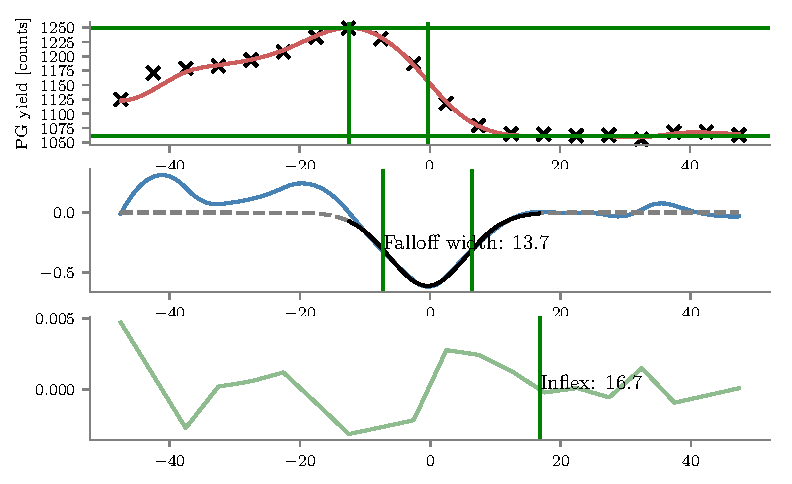
\includegraphics[width=.45\textwidth]{FOW_PMMA_phantom-iba-auger-tof-3}}\quad
  \subfloat[MPS]{\label{FOWMPS}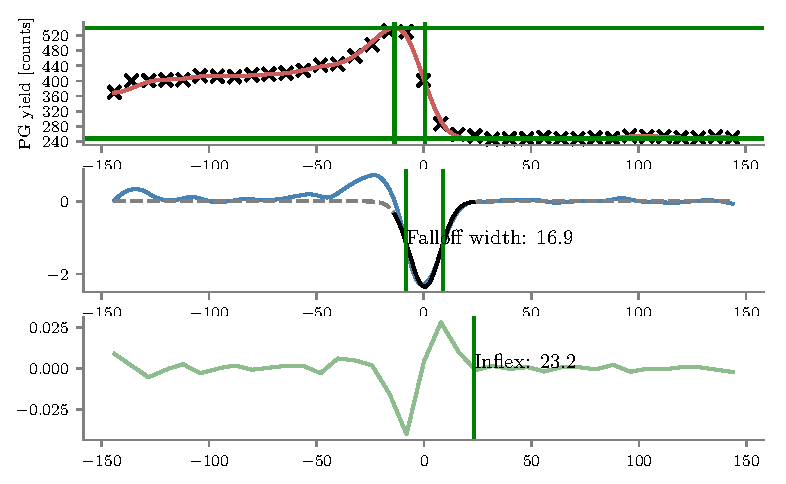
\includegraphics[width=.45\textwidth]{FOW_PMMA_phantom-ipnl-auger-tof-3}}
  \caption{\label{FOWILLUS} MPS and KES FOW estimation illustrated. \ds{idem x scale}}
\end{figure}

Figure~\ref{FOWILLUS} shows and illustration of the procedure for two selected profiles obtained with each collimator. To estimate the fall-off width (FOW), we smooth the profile in a similar manner as for the FOP estimation, as detailed in appendix~\ref{sec:fopproc} (row 1 in Figure~\ref{FOWILLUS}). Then, a first and second order derivative is computed. On the first order derivative, a Gaussian is fitted (dashed line on second row), on the interval (solid line) between the profile maximum (Bragg Peak) and the first inflection point past the FOP on the second order derivative (here the 1D PG profile is at the baseline of the background, see third row). The Gaussian is fit with a fixed offset of zero, because the baseline of the background is zero. The full width half max of the fitted Gaussian is then taken as the FOW (second row).

%%%%%%%%%%%%%%%%%%%%%%%%%%%%%%%%%%%%%%%%%%%%%%%%%%%%%%%%%%%%%%%%%%%%%%%%%%%%%%%%

\section{Verification of the cameras}

In \cite{Priegnitz2015} PG shifts due to beam energy shifts are studied for the KES camera: the \emph{detectability} of the fall-off as function of the number of primaries. Here that simulation was recreated: a mono-energetic beam shoots into a waterbox at two energies. 50 realizations are generated with a 139 MeV beam energy, and 50 realizations with 144 MeV. At $10^9$ primaries, the distributions are well separated with a shift of 8.3 mm (different from \cite{Priegnitz2015} because of the different material). In figure 13 in \cite{Perali2014} with $10^9$ primaries a standard deviation of 1.5 mm is obtained, while here 1.21 and 1.14 mm were obtained. It is sufficient agreement to be confident of our setup and further results.

The KES prototype's sensitivity to accurate positioning with respect to the expected FOP was elaborated upon in \citet[Section IV.A.3]{Sterpin2015}: the detector response is, due to the KES collimator, not linear as with a parallel slit collimator. In this study, to make the comparison as fair as possible and avoid any bias, alignment on the FOP specific for each spot was ensured as follows: the intermediate PG source image of vpgTLE (equivalent to the PG emission) was projected on the beam axis, and then convolved with a Gaussian of $\upsigma = 8.5$ mm, which corresponds to the point spread function (PSF) with a FWHM of 20 mm used in \cite{Priegnitz2015} to approximate the detected profiles from the emitted profile. These profiles will be referred to as \qq{PG + PSF} profiles. As a matter of fact, the MPS prototype has roughly the same PSF as the KES prototype so that \qq{PG + PSF} fall-off position can be considered as the expected position for both cameras.

To verify the implementation of the MPS camera, the precision on the FOP, obtained with the procedure outlined in the previous paragraph, is compared to earlier results. In the caption of figure 9 in \cite{Pinto2014a} it is stated that with $10^8$ primaries a standard deviation of 1.3 mm is obtained for the detector design used here, which is about 20\% different from the results obtained in this study: 1.63 and 1.54 mm.
%%%%%%%%%%%%%%%%%%%%%%%%%%%%%%%%%%%%%%%%%%%%%%%%%%%%%%%%%%%%%%%%%%%%%%%%%%%%%%%%
% \end{appendices}
\newpage

%%%%%%%%%%%%%%%%%%%%%%%%%%%%%%%%%%%%%%%%%%%%%%%%%%%%%%%%%%%%%%%%%%%%%%%%%%%%%%%%

\bibliographystyle{plainnat}
\bibliography{lib.bib}
\end{document}%\grid
